\icode{E-MC-SI-L2-2624-001}
小明同学要过一条\,\qty{60}{m}宽、河岸平直的小河，所乘小船在静水中划行速率为\,\qty{3}{m/s}，河水流速为\,\qty{5}{m/s}，下列判断正确的是\paren[]

\begin{choices}
	\item 过河最短时间为\,\qty{12}{s}
	\item 过河最短时间为\,\qty{20}{s}
	\item 过河最短位移为\,\qty{60}{m}
	\item 过河最短位移为\,\qty{80}{m}
\end{choices}
\begin{answer}
	B\quad 提示：最短位移\,\qty{100}{m}
	
	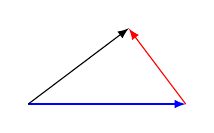
\begin{tikzpicture}[font=\scriptsize,>=latex]
		\draw[->,blue] (0,0)--(2,0);
		\draw[->,red] (2,0)--++(127:1.2);
		\draw[->] (0,0)--(37:1.6);
	\end{tikzpicture}
\end{answer}
